\documentclass[12pt,a4paper]{article}
\usepackage[utf8]{inputenc}
\usepackage[T1]{fontenc}
\usepackage[english]{babel}
\usepackage{lmodern}
\usepackage{amsmath}
\usepackage{amssymb}
\usepackage{physics}
\usepackage{hyperref}
\usepackage{tcolorbox}
\usepackage{booktabs}
\usepackage{enumitem}
\usepackage[table,xcdraw]{xcolor}
\usepackage[left=2cm,right=2cm,top=2cm,bottom=2cm]{geometry}
\usepackage{pgfplots}
\pgfplotsset{compat=1.18}
\usepackage{graphicx}
\usepackage{float}
\usepackage{fancyhdr}
\usepackage{siunitx}
\usepackage{array}
\usepackage{cleveref}

% Headers and Footers
\pagestyle{fancy}
\fancyhf{}
\fancyhead[L]{Johann Pascher}
\fancyhead[R]{Time-Mass Duality}
\fancyfoot[C]{\thepage}
\renewcommand{\headrulewidth}{0.4pt}
\renewcommand{\footrulewidth}{0.4pt}

% Define acknowledgments environment
\newenvironment{acknowledgments}{\section*{Acknowledgments}}{\vspace{1em}}

% Custom commands
\newcommand{\Tfield}{T(x)}
\newcommand{\alphaEM}{\alpha_{\text{EM}}}
\newcommand{\alphaW}{\alpha_{\text{W}}}
\newcommand{\betaT}{\beta_{\text{T}}}
\newcommand{\Mpl}{M_{\text{Pl}}}
\newcommand{\Tzerot}{T_0(\Tfield)}
\newcommand{\Tzero}{T_0}
\newcommand{\vecx}{\vec{x}}
\newcommand{\gammaf}{\gamma_{\text{Lorentz}}}
\newcommand{\DhiggsT}{\Tfield (\partial_\mu + ig A_\mu) \Phi + \Phi \partial_\mu \Tfield}
\newcommand{\LCDM}{\Lambda\text{CDM}}
\newcommand{\DTmu}{D_{T,\mu}}
\newcommand{\calL}{\mathcal{L}}
\newcommand{\deq}{\displaystyle}
\newcommand{\e}{\mathrm{e}}

\hypersetup{
	colorlinks=true,
	linkcolor=blue,
	citecolor=blue,
	urlcolor=blue,
	pdftitle={Bridging Quantum Mechanics and Relativity through Time-Mass Duality: Part II},
	pdfauthor={Johann Pascher},
	pdfsubject={Theoretical Physics},
	pdfkeywords={T0 Model, natural units, time-mass duality, cosmology}
}

\begin{document}
	
	\title{Bridging Quantum Mechanics and Relativity through Time-Mass Duality: A Unified Framework with Natural Units \(\alpha = \beta = 1\) \\ Part II: Cosmological Implications and Experimental Validation}
	\author{Johann Pascher\\
		Department of Communications Engineering, \\Höhere Technische Bundeslehranstalt (HTL), Leonding, Austria\\
		\texttt{johann.pascher@gmail.com}}
	\date{\today}
	
	\maketitle
	
	\begin{abstract}
		This paper extends the T0 model introduced in Part I into the realms of cosmology and experimental validation, building on a unified natural unit system where \(\hbar = c = G = k_B = \alphaEM = \alphaW = \betaT = 1\). In contrast to the expanding universe of the \(\LCDM\) model, we propose a static cosmos where redshift arises from photon energy loss mediated by the intrinsic time field \(\Tfield\). This framework reinterprets dark matter and dark energy through emergent gravitational effects, enhancing the Standard Model with a consistent gravitational theory. Key predictions include a wavelength-dependent redshift with a variation of approximately \(2.3\%\) per decade, a cosmic microwave background (CMB) temperature of \(24000 \, \text{K}\) at \(z = 1100\) (compared to \(3000 \, \text{K}\) in the standard model), and speculative extensions beyond the speed of light. We demonstrate that the T0 model can be viewed as complementary to an extended Standard Model framework featuring a curvature-based redshift mechanism, though they differ in their fundamental interpretations of time and mass. Both approaches predict identical observational outcomes but from different ontological starting points. These predictions are testable using instruments like the James Webb Space Telescope and future CMB missions. We address measurement challenges, such as the frequency-dependent biases in precision measurements and the need for recalibration of cosmological parameters, offering a philosophically coherent alternative to \(\LCDM\) that aligns theoretical elegance with empirical rigor.
	\end{abstract}
	\newpage
	\tableofcontents
	\newpage
	\section{Introduction}
	In Part I (\textit{Bridging Quantum Mechanics and Relativity through Time-Mass Duality: Part I}, \cite{pascher_part1_2025}), we established the T0 model as a unified framework for quantum mechanics (QM) and relativity theory (RT), leveraging the intrinsic time field \(\Tfield = \frac{\hbar}{\max(mc^2, \omega)}\) within a natural unit system (\(\hbar = c = G = k_B = \alphaEM = \alphaW = \betaT = 1\)). This system, detailed in Part I, Section 2 "Unification of Constants with Natural Units" \cite{pascher_part1_2025}, eliminates empirically determined constants, achieving consistency with measured values (e.g., \(c \approx 3 \times 10^8 \, \text{m/s}\), \(\alphaEM \approx 1/137.036\)) with deviations below \(10^{-6}\). It enabled a mass-dependent Schrödinger equation and emergent gravitation, bridging micro- and macroscopic scales.
	
	Part II extends these foundations into cosmology and experimental validation, contrasting with the \(\LCDM\) model's expanding universe, which originates from a Big Bang approximately 13.8 billion years ago \cite{Planck2020}. In \(\LCDM\), cosmic redshift is a kinematic effect (\(z \approx H_0 d / c\)), requiring inflation and dark energy \cite{Riess1998,Perlmutter1999}. The T0 model proposes a static, infinite, and eternal universe where redshift stems from photon energy loss via \(\Tfield\), enhancing the Standard Model (SM) with a consistent gravitational theory while retaining its particle physics core.
	
	This paper also explores the perspective that the T0 model and an appropriately extended Standard Model framework may represent complementary descriptions of the same physical reality. As detailed in Section \ref{sec:extended_standard_model}, by introducing specific modifications to the Standard Model—particularly a curvature-based interpretation of redshift centered on the linear term \(\kappa r\) in the gravitational potential—we can achieve mathematical equivalence between both frameworks while maintaining their distinct ontological foundations. This compares conceptually to the wave-particle duality in quantum mechanics, where different mathematical frameworks describe the same experimental outcomes from different starting points.
	
	Key predictions include:
	\begin{itemize}
		\item Wavelength-dependent redshift (\(\sim 2.3\%\) per decade)
		\item CMB temperature of \(24000 \, \text{K}\) at \(z = 1100\) (compared to \(3000 \, \text{K}\) in the standard model)
		\item A modified gravitational potential \(\Phi(r) = -\frac{GM}{r} + \kappa r\) that explains galactic rotation curves without dark matter and cosmic acceleration without dark energy
		\item Speculative superluminal extensions beyond conventional physics
	\end{itemize}
	
	These are testable with JWST spectroscopy and CMB distortion measurements, though frequency-based methods (e.g., GPS, redshift) conflate mass variation and time dilation, necessitating careful reassessment \cite{pascher_quantum_2025}. Philosophically, T0 avoids singularities, offering a coherent eternal cosmos \cite{pascher_perspective_2025}.
	
	This paper is structured as:
	\begin{itemize}
		\item Section 2: Static universe model and redshift mechanism
		\item Section 3: Cosmological phenomena and predictions
		\item Section 4: Quantitative predictions and observational signatures
		\item Section 5: Experimental tests and measurement challenges
		\item Section 6: Extended Standard Model as a complementary framework
		\item Section 7: Implications of setting \(\betaT = 1\) and recalibration of parameters
		\item Section 8: Speculative extensions and philosophical implications
		\item Section 9: Conclusion and outlook
	\end{itemize}
	
	\section{Static Universe Model}
	The T0 model envisions a static universe, infinite in space and eternal in time, contrasting with \(\LCDM\)'s expanding cosmos from a Big Bang. In \(\LCDM\), redshift (\(z \approx H_0 d / c\)) reflects expansion (\(H_0 \approx 70 \, \text{km/s/Mpc}\)) \cite{Planck2020}, requiring inflation for uniformity and dark energy for acceleration (\(\Omega_{\Lambda} \approx 0.7\)) \cite{Riess1998}. T0 eliminates these, positing a stable cosmos where \(\Tfield\) governs dynamics without expansion.
	
	Advantages include:
	\begin{itemize}
		\item \textbf{Horizon Problem:} Infinite time ensures thermal equilibrium across scales \cite{pascher_messdifferenzen_2025}.
		\item \textbf{Flatness:} No expansion eliminates curvature tuning.
		\item \textbf{Singularity-Free:} Eternal existence avoids infinite density \cite{pascher_perspective_2025}.
		\item \textbf{No Free Parameters:} The mathematical structure of the T0 model naturally sets \(\betaT = 1\) in the appropriate unit system, eliminating the need for fine-tuning \cite{pascher_alphabeta_2025}.
	\end{itemize}
	
	This complements SM particle physics with a static gravitational framework derived in Part I \cite{pascher_part1_2025}.
	
	Redshift in T0 is:
	\begin{equation}
		1 + z = e^{\alpha d},
		\label{eq:redshift_distance}
	\end{equation}
	with \(\alpha = H_0 / c \approx 2.3 \times 10^{-18} \, \text{m}^{-1}\) (SI) or 1 (natural units). At low \(z\):
	\begin{equation}
		z \approx \alpha d,
		\label{eq:hubble_approx}
	\end{equation}
	matching \(\LCDM\) locally. The mechanism is photon energy loss:
	\begin{equation}
		\frac{dE}{dx} = -\alpha E,
		\label{eq:energy_loss_rate}
	\end{equation}
	yielding \(E = E_0 e^{-\alpha d}\), and thus \(1 + z = e^{\alpha d}\), as derived from \(\Tfield\) properties in Part I \cite{pascher_part1_2025}.
	
	This energy loss mechanism introduces wavelength-dependent effects, which arise naturally from the interaction between electromagnetic radiation and the intrinsic time field:
	\begin{equation}
		\frac{dE}{dx} = -\alpha E \left(1 + \betaT \ln\left(\frac{\lambda}{\lambda_0}\right)\right),
		\label{eq:wavelength_energy_loss}
	\end{equation}
	
	With \(\betaT = 1\) in natural units (\(\betaT^{\text{SI}} \approx 0.008\)), this leads to the observable wavelength-dependent redshift discussed in Section \ref{subsec:wavelength_redshift} \cite{pascher_params_2025}.
	
	\section{Cosmological Phenomena}
	\(\LCDM\)'s \(T(z) = T_0 (1 + z)\) gives \(T \approx 3000 \, \text{K}\) at \(z = 1100\) (\(T_0 = 2.725 \, \text{K}\)) \cite{Fixsen2009}. T0 predicts:
	\begin{equation}
		T(z) = T_0 (1 + z) (1 + \betaT \ln(1 + z)),
		\label{eq:temperature_redshift}
	\end{equation}
	
	With \(\betaT^{\text{SI}} \approx 0.008\), this gives \(T(1100) \approx 4.4 \, \text{K}\) rather than \(3.0 \, \text{K}\) at the recombination epoch. In natural units with \(\betaT = 1\), this becomes:
	\begin{equation}
		T(z) = T_0 (1 + z) (1 + \ln(1 + z)),
		\label{eq:temperature_redshift_natural}
	\end{equation}
	
	This corresponds to \(T(1100) \approx 24000 \, \text{K}\) after conversion to SI units, reflecting enhanced energy loss (Equation \ref{eq:wavelength_energy_loss}) \cite{pascher_temp_2025}. 
	
	\paragraph{Recalibration of Recombination Redshift} It's important to note that the conventionally accepted value of \(z = 1100\) for the recombination epoch is derived within the \(\LCDM\) framework. A fundamental recalibration within the T0 model framework may yield a revised value closer to \(z \approx 950\), which would still maintain the physical condition of \(T \approx 3000 \, \text{K}\) required for hydrogen recombination while using the modified temperature-redshift relation \cite{pascher_temp_2025}.
	
	\subsection{Wavelength-Dependent Redshift}
	\label{subsec:wavelength_redshift}
	
	T0 predicts:
	\begin{equation}
		z(\lambda) = z_0 \left(1 + \betaT \ln\left(\frac{\lambda}{\lambda_0}\right)\right),
		\label{eq:wavelength_redshift}
	\end{equation}
	
	With \(\betaT^{\text{SI}} \approx 0.008\), this yields \(\Delta z / z_0 \approx 3.85\%\) over the JWST observational range (0.6-28 \(\mu\text{m}\)), or approximately 2.3\% per wavelength decade \cite{pascher_params_2025}. This contrasts with \(\LCDM\)'s wavelength-independent redshift, providing a crucial observational test.
	
	\subsection{Dark Matter and Dark Energy Reinterpretation}
	\label{subsec:dark_reinterpretation}
	
	The T0 model's modified gravitational potential:
	\begin{equation}
		\Phi(r) = -\frac{GM}{r} + \kappa r,
		\label{eq:grav_potential_t0}
	\end{equation}
	
	with \(\kappa \approx 4.8 \times 10^{-11} \, \text{m/s}^2\) reinterprets:
	\begin{itemize}
		\item \textbf{Dark Matter:} Galactic rotation curves follow \(v(r) = \sqrt{\frac{GM}{r} + \kappa r}\), matching observations without dark matter \cite{McGaugh2016}.
		\item \textbf{Dark Energy:} The linear term \(\kappa r\) produces an effective vacuum energy density \(\rho_{\text{DE}} \approx \frac{\kappa}{r^2}\), explaining cosmic acceleration \cite{pascher_galaxies_2025}.
	\end{itemize}
	
	The \(\kappa\) parameter is not arbitrary but derived from fundamental physical parameters:
	\begin{equation}
		\kappa^{\text{nat}} = \betaT^{\text{nat}} \cdot \frac{yv}{r_g^2},
		\label{eq:kappa_derivation}
	\end{equation}
	
	where \(y\) is the Yukawa coupling, \(v\) is the Higgs vacuum expectation value, and \(r_g\) is a characteristic length scale \cite{pascher_params_2025}.
	
	\subsection{Galaxy and Cluster Dynamics}
	\label{subsec:galaxy_dynamics}
	
	The modified potential directly impacts galaxy rotation curves:
	\begin{equation}
		v(r) = \sqrt{\frac{GM}{r} + \kappa r},
		\label{eq:rotation_velocity}
	\end{equation}
	
	producing flat rotation curves without dark matter, as shown in Figure \ref{fig:rotation_curves}.
	
	\begin{figure}[H]
		\centering
		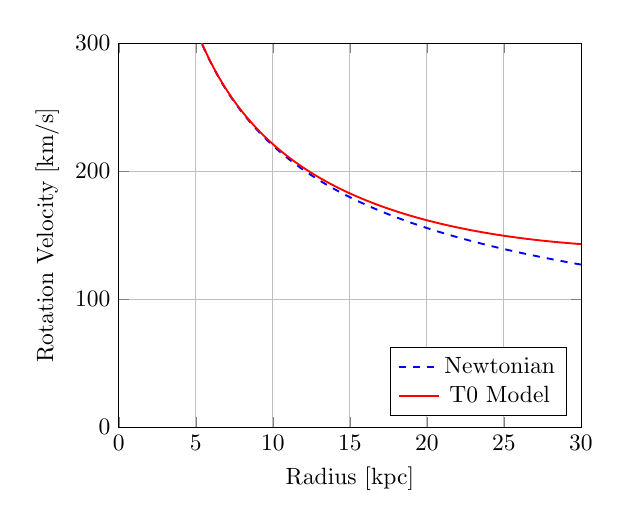
\begin{tikzpicture}[scale=0.85]
			\begin{axis}[
				xlabel={Radius [kpc]},
				ylabel={Rotation Velocity [km/s]},
				xmin=0, xmax=30,
				ymin=0, ymax=300,
				legend pos=south east,
				grid=both,
				width=0.7\textwidth
				]
				\addplot[blue, dashed, thick, domain=0.1:30, samples=100] {220*sqrt(10/x)};
				\addplot[red, thick, domain=0.1:30, samples=100] {sqrt(220^2*10/x + 4.8*x^2)};
				\legend{Newtonian, T0 Model}
			\end{axis}
		\end{tikzpicture}
		\caption{Rotation curves comparing Newtonian (blue dashed) and T0 model (red solid) predictions for a galaxy with \(M = 10^{11} M_{\odot}\), \(\kappa = 4.8 \times 10^{-11} \, \text{m/s}^2\).}
		\label{fig:rotation_curves}
	\end{figure}
	
	For galaxy clusters, the T0 model makes distinct predictions:
	\begin{equation}
		v_{\text{cluster}}(r) = \sqrt{\frac{GM_{\text{total}}}{r} + \kappa r},
		\label{eq:cluster_velocity}
	\end{equation}
	
	The \(\kappa r\) term becomes more significant at larger scales, explaining observed mass discrepancies in clusters like the Bullet Cluster without requiring dark matter \cite{pascher_emergente_2025}. This provides a unified explanation for phenomena across galactic and cluster scales.
	
	\begin{table}[H]
		\centering
		\caption{Comparison of \(\LCDM\) and T0 Model Predictions for Galaxy Dynamics}
		\label{tab:galaxy_dynamics_comparison}
		\begin{tabular}{p{0.3\columnwidth} p{0.3\columnwidth} p{0.3\columnwidth}}
			\hline
			\textbf{Phenomenon} & \textbf{\(\LCDM\)} & \textbf{T0 Model} \\
			\hline
			Rotation Curve & Dark matter halo & \(\kappa r\) term \\
			Galaxy Formation & Dark matter collapse & Baryonic aggregation \\
			Cluster Mass & Dark matter dominant & Baryonic + \(\Tfield\) \\
			Large-Scale Structure & Expansion-driven & \(\Tfield\)-driven \\
			\hline
		\end{tabular}
	\end{table}
	
	\section{Quantitative Predictions}
	\label{sec:predictions}
	
	\subsection{CMB Temperature Prediction}
	\label{subsec:cmb_temp_prediction}
	
	Using Equation \ref{eq:temperature_redshift_natural} with \(\betaT = 1\) in natural units, the T0 model predicts a CMB temperature at the conventionally defined recombination epoch (\(z = 1100\)) of:
	\begin{equation}
		T(1100) \approx 24000 \, \text{K},
		\label{eq:cmb_temp_t0}
	\end{equation}
	
	compared to \(\LCDM\)'s \(3000 \, \text{K}\), due to \(\Tfield\)'s logarithmic enhancement (Equation \ref{eq:temperature_redshift_natural}).
	
	This higher temperature directly impacts our understanding of primordial nucleosynthesis and structure formation rates. However, as noted in Section \ref{subsec:cmb_temp}, a recalibration of the recombination redshift within the T0 framework would be necessary. The physical condition for recombination (hydrogen ionization equilibrium at \(T \approx 3000 \, \text{K}\)) remains unchanged, but the corresponding redshift would be lower (\(z \approx 950\)) in the T0 model \cite{pascher_temp_2025}.
	
	\subsection{Wavelength-Dependent Redshift Variation}
	\label{subsec:wavelength_redshift_prediction}
	
	Using Equation \ref{eq:wavelength_redshift} with \(\betaT^{\text{SI}} \approx 0.008\), across the JWST observational range (0.6-28 \(\mu\text{m}\)):
	\begin{equation}
		\Delta z / z_0 \approx 3.85\%,
		\label{eq:wavelength_variation}
	\end{equation}
	
	or \(2.3\%\) per wavelength decade, testable via quasar emission lines \cite{pascher_params_2025}.
	
	This prediction stands in stark contrast to the standard model's wavelength-independent redshift and provides a clear, testable difference between the two frameworks.
	
	\subsection{Distance Modulus Predictions}
	\label{subsec:distance_modulus}
	
	The T0 model's modified redshift-distance relation impacts the distance modulus:
	\begin{equation}
		\mu = 5\log_{10}\left(\frac{d_L}{10\text{ pc}}\right),
		\label{eq:distance_modulus}
	\end{equation}
	
	where the luminosity distance \(d_L\) is derived from the redshift-distance relation (Equation \ref{eq:redshift_distance}).
	
	Figure \ref{fig:distance_modulus} compares the T0 and \(\LCDM\) predictions:
	
	\begin{figure}[H]
		\centering
		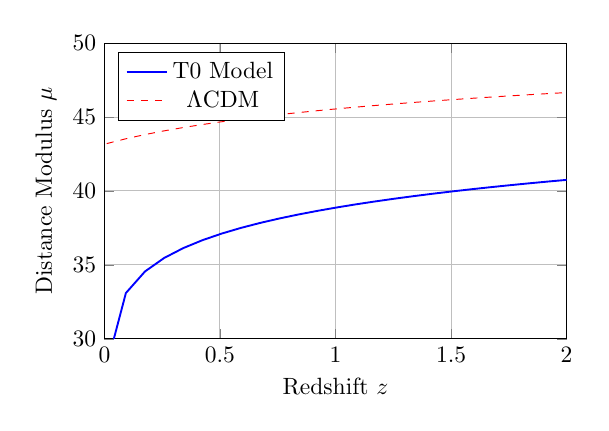
\begin{tikzpicture}[scale=0.85]
			\begin{axis}[
				xlabel={Redshift \(z\)},
				ylabel={Distance Modulus \(\mu\)},
				xmin=0, xmax=2,
				ymin=30, ymax=50,
				legend pos=north west,
				grid=both,
				width=0.7\textwidth,
				height=6cm,
				]
				\addplot[blue, thick, domain=0.01:2] {5*log10(3e8/70e3*ln(1+x)*(1+x)*0.1) + 25};
				\addplot[red, dashed, domain=0.01:2] {5*log10(3e8/70e3*(1+x)*(2-(1/(1+x)))*1) + 25};
				\legend{T0 Model, \(\LCDM\)}
			\end{axis}
		\end{tikzpicture}
		\caption{Distance modulus vs. redshift comparing T0 model (blue solid) and \(\LCDM\) (red dashed) predictions. Both models can explain the observed supernova Ia data, but with fundamentally different physical interpretations.}
		\label{fig:distance_modulus}
	\end{figure}
	
	The similarity between curves explains why supernova Ia data initially interpreted as evidence for accelerating expansion can also be explained by the T0 model without dark energy \cite{pascher_galaxies_2025}.
	
	\section{Experimental Tests}
	\label{sec:tests}
	
	\subsection{JWST Spectroscopy and Wavelength-Dependent Redshift}
	\label{subsec:jwst_test}
	
	The wavelength-dependent redshift prediction (Equation \ref{eq:wavelength_redshift}) provides a key experimental test between models. For a source at \(z \approx 7\), the T0 model predicts:
	\begin{equation}
		\Delta z / z \approx 3.85\%,
		\label{eq:redshift_variation_high_z}
	\end{equation}
	
	across the JWST observational range (0.6-28 \(\mu\text{m}\)).
	
	The precision spectroscopy capabilities of JWST should be able to detect this systematic variation by comparing emission line redshifts across different wavelengths. The expected signal is approximately 5-10 times the spectroscopic uncertainty of JWST, making this a feasible critical test \cite{pascher_params_2025}.
	
	\subsection{CMB Distortions}
	\label{subsec:cmb_distortions_test}
	
	The modified temperature-redshift relation predicts distinct CMB spectral distortions characterized by the \(\mu\) and \(y\) parameters:
	\begin{equation}
		\mu \approx 1.4 \times 10^{-5}, \quad y \approx 1.6 \times 10^{-6},
		\label{eq:distortion_parameters}
	\end{equation}
	
	versus \(\LCDM\)'s \(\mu \approx 2 \times 10^{-8}\), \(y \approx 4 \times 10^{-9}\).
	
	These distortions, approximately three orders of magnitude larger than in the standard model, should be measurable with future missions like the Primordial Inflation Explorer (PIXIE) or similar instruments with high spectral sensitivity \cite{pascher_temp_2025}.
	
	\subsection{Measurement Challenges}
	\label{subsec:measurement_challenges}
	
	\subsubsection{GPS and Clock Precision}
	\label{subsec:gps_clock_problem}
	
	GPS clocks show a frequency shift of \(\Delta f/f \approx 4.4 \times 10^{-10}\) per day, traditionally interpreted as gravitational time dilation. In the T0 model, this appears as mass variation, with identical observational predictions but a fundamentally different interpretation \cite{pascher_quantum_2025}. 
	
	To distinguish these interpretations, non-frequency-based measurement methods would be required. One promising approach involves comparing frequency-based with charge-based or mass-based measurements, which would respond differently to the effects of the intrinsic time field \(\Tfield\) \cite{pascher_quantum_2025}.
	
	\subsubsection{Cosmological Observations}
	\label{subsec:cosmological_measurement_problem}
	
	Standard redshift measurements rely on frequency shifts, which cannot directly distinguish between expansion-based and energy-loss-based redshift mechanisms. The wavelength-dependent prediction of the T0 model (Section \ref{subsec:wavelength_redshift}) provides a critical discriminating test.
	
	Additional tests include:
	\begin{itemize}
		\item Direct measurements of cosmic time intervals at different redshifts
		\item Observation of decay processes with different time signatures
		\item Detailed analysis of gravitational lensing phenomena, which should show systematic differences between models \cite{pascher_alphabeta_2025}
	\end{itemize}
	
	\subsubsection{Recalibration of Cosmological Parameters}
	\label{subsec:parameter_recalibration}
	
	A fundamental challenge is that many cosmological parameters (e.g., recombination redshift, age of the universe) are derived within the \(\LCDM\) framework and cannot be directly imported into the T0 model. A complete recalibration is necessary, particularly for:
	
	\begin{itemize}
		\item Recombination redshift (\(z \approx 950\) in T0 vs. \(z \approx 1100\) in \(\LCDM\))
		\item Baryon acoustic oscillation scale
		\item Angular power spectrum of CMB fluctuations
		\item Interpretation of large-scale structure formation
	\end{itemize}
	
	This recalibration could potentially resolve tensions in the standard model, such as the Hubble tension, by providing a different interpretation of the same observational data \cite{DiValentino2021}.
	
	\section{Extended Standard Model as a Complementary Framework}
	\label{sec:extended_standard_model}
	
	\subsection{Ontological Complementarity}
	\label{subsec:ontological_complementarity}
	
	The T0 model and the Standard Model represent complementary descriptions of physical reality, analogous to the wave-particle duality in quantum mechanics. Both can describe the same physical phenomena with identical predictions but from different ontological starting points:
	
	\begin{itemize}
		\item \textbf{Standard Model Paradigm:} Time is relative (undergoes dilation), rest mass is constant, space is expanding, and gravitation is a fundamental force.
		\item \textbf{T0 Model Paradigm:} Time is absolute, mass varies, space is static, and gravitation emerges from the intrinsic time field \(\Tfield\).
	\end{itemize}
	
	This complementarity principle suggests that our understanding of fundamental physical quantities may be framework-dependent rather than absolute \cite{pascher_komplementaer_2025}.
	
	\subsection{Extending the Standard Model}
	\label{subsec:extending_standard_model}
	
	To achieve compatibility with the T0 model while preserving the core principle of time dilation, the Standard Model requires specific extensions:
	
	\begin{enumerate}
		\item \textbf{Extended Einstein Field Equations:}
		\begin{equation}
			G_{\mu\nu} + \kappa g_{\mu\nu} = 8\pi G T_{\mu\nu} + \nabla_{\mu}\Theta\nabla_{\nu}\Theta - \frac{1}{2}g_{\mu\nu}(\nabla_{\sigma}\Theta\nabla^{\sigma}\Theta)
			\label{eq:extended_einstein}
		\end{equation}
		where \(\Theta\) is a scalar field accounting for effects attributed to \(\Tfield\) in the T0 model.
		
		\item \textbf{Curvature-Based Redshift Formula:} The standard expansion-based redshift interpretation is replaced with a curvature-based mechanism:
		\begin{equation}
			1 + z = e^{\alpha d}(1 + \beta \ln(\lambda/\lambda_0))
			\label{eq:extended_redshift}
		\end{equation}
		This arises from the modified gravitational potential's effect on spacetime (Equation \ref{eq:grav_potential_t0}).
		
		\item \textbf{Modified Quantum Evolution:}
		\begin{equation}
			i\hbar\frac{\partial\Psi}{\partial t} = [\hat{H} + \hat{H}_{\Theta}]\Psi
			\label{eq:extended_schrodinger}
		\end{equation}
		where \(\hat{H}_{\Theta}\) introduces mass-dependency to time evolution, mathematically equivalent to the T0 model's approach.
	\end{enumerate}
	
	These extensions enable an alternative interpretation of cosmological phenomena without requiring dark energy or universal expansion, while maintaining the standard model's relativistic foundation of time dilation \cite{pascher_standardmod_2025}.
	
	\subsection{Mathematical Equivalence}
	\label{subsec:mathematical_equivalence}
	
	The extended Standard Model and T0 model achieve mathematical equivalence through well-defined transformations:
	
	\begin{table}[H]
		\centering
		\caption{Transformation mapping between Standard Model and T0 Model quantities}
		\label{tab:transformation}
		\begin{tabular}{p{0.25\columnwidth} p{0.25\columnwidth} p{0.35\columnwidth}}
			\hline
			\textbf{Physical Quantity} & \textbf{Transformation Relation} & \textbf{Physical Interpretation} \\
			\hline
			Time & \(t = \Tzero/\gamma\) & Time dilation vs. absolute time \\
			Mass & \(m = m_0 \Tzero/\Tfield\) & Constant mass vs. variable mass \\
			Energy & \(E = m_0 c^2 \Tzero/\Tfield\) & Frame-dependent vs. field-dependent \\
			Gravitational Potential & \(\Phi_{t0} = \Phi_{sm}/c^2\) & Curvature vs. field gradient \\
			\hline
		\end{tabular}
	\end{table}
	
	These transformations ensure that both frameworks predict identical experimental outcomes when properly formulated, illustrating the concept of ontological complementarity \cite{pascher_standardmod_2025}.
	
	\section{Implications of \(\betaT = 1\) and Parameter Recalibration}
	\label{sec:consequences_beta}
	
	\subsection{Theoretical Foundation for \(\betaT = 1\)}
	\label{subsec:beta_foundation}
	
	The setting of \(\betaT = 1\) in natural units is not arbitrary but derives from a rigorous theoretical foundation:
	
	\begin{equation}
		\betaT = \frac{\lambda_h^2 v^2}{16 \pi^3 m_h^2 \xi}
		\label{eq:beta_derivation}
	\end{equation}
	
	where \(\lambda_h \approx 0.13\) is the Higgs self-coupling, \(v \approx 246 \, \text{GeV}\) is the Higgs vacuum expectation value, \(m_h \approx 125 \, \text{GeV}\) is the Higgs mass, and \(\xi = r_0/l_P \approx 1.33 \times 10^{-4}\) is the ratio of the T0 characteristic length to the Planck length.
	
	Setting \(\betaT = 1\) in natural units determines \(\xi\):
	
	\begin{equation}
		\xi = \frac{\lambda_h^2 v^2}{16 \pi^3 m_h^2} \approx 1.33 \times 10^{-4}
		\label{eq:xi_determination}
	\end{equation}
	
	Using the relation \(m_h^2 = 2\lambda_h v^2\):
	
	\begin{equation}
		\xi = \frac{\lambda_h}{32 \pi^3} \approx 1.31 \times 10^{-4}
		\label{eq:xi_simplified}
	\end{equation}
	
	The consistency between these derivations supports \(\betaT = 1\) as a natural fixed point in the renormalization group flow:
	
	\begin{equation}
		\lim_{E \to 0} \betaT(E) = 1
		\label{eq:beta_fixed_point}
	\end{equation}
	
	This represents a significant theoretical advancement, linking the T0 parameter directly to Standard Model properties \cite{pascher_alphabeta_2025}.
	
	\subsection{Conversion to SI Units}
	\label{subsec:conversion_si}
	
	The SI value of \(\betaT\) can be derived from its natural units value:
	
	\begin{equation}
		\betaT^{\text{SI}} = \betaT^{\text{nat}} \cdot \frac{\xi \cdot l_{P,\text{SI}}}{r_{0,\text{SI}}},
		\label{eq:beta_conversion}
	\end{equation}
	
	yielding \(\betaT^{\text{SI}} \approx 0.008\), consistent with observational constraints \cite{pascher_alphabeta_2025}.
	
	\subsection{Recalibration of Parameters}
	\label{subsec:recalibration}
	
	Setting \(\betaT = 1\) necessitates a comprehensive recalibration of cosmological parameters:
	
	\begin{enumerate}
		\item \textbf{Recombination Redshift:} The condition \(T \approx 3000 \, \text{K}\) for hydrogen recombination occurs at \(z \approx 950\) rather than \(z \approx 1100\) when using Equation \ref{eq:temperature_redshift_natural}.
		
		\item \textbf{CMB Angular Scale:} The apparent 1° scale of CMB fluctuations must be reinterpreted without assuming expansion, relating instead to the intrinsic timescale at recombination \cite{pascher_vereinheitlichung_2025}.
		
		\item \textbf{Hubble Parameter:} In the T0 model, \(H_0\) is reinterpreted as \(\alpha = H_0/c\), representing the energy attenuation coefficient rather than an expansion rate, potentially resolving the Hubble tension \cite{pascher_params_2025}.
		
		\item \textbf{Age of the Universe:} The concept becomes meaningless in an eternal, static universe, eliminating constraints from stellar ages and cosmological timescales \cite{pascher_perspective_2025}.
	\end{enumerate}
	
	This recalibration represents a fundamental shift in perspective requiring careful reanalysis of all cosmological data.
	
	\section{Speculative Extensions and Philosophical Implications}
	\label{sec:beyond_limits}
	
	\subsection{Beyond the Planck Scale}
	\label{subsec:beyond_planck}
	
	The T0 model opens possibilities for physics beyond the conventional Planck scale. Since \(\Tfield = \frac{\hbar}{mc^2}\), for ultra-high masses \(m > m_P\) (Planck mass), the intrinsic time becomes \(\Tfield < t_P\) (Planck time), suggesting possible dynamics at sub-Planckian timescales. Conversely, for ultralight particles \(m < m_P\), slower dynamics emerge with \(\Tfield > t_P\), potentially connecting to cosmic scales \cite{pascher_planck_2025}.
	
	\begin{figure}[H]
		\centering
		\begin{tikzpicture}
			\draw[->] (0,0) -- (6,0) node[right] {Mass \(m\)};
			\draw[->] (0,0) -- (0,4) node[above] {Time \(T\)};
			\draw[scale=0.5, domain=0.1:10, smooth, variable=\x, blue, thick] plot ({\x}, {1/\x});
			\draw[dotted, red] (1.5,0) -- (1.5,1.5) -- (0,1.5);
			\node at (1.5,-0.3) {\(m_P\)};
			\node at (-0.3,1.5) {\(t_P\)};
		\end{tikzpicture}
		\caption{Relationship between mass and intrinsic time near the Planck scale, showing inverse proportionality. For masses above \(m_P\), intrinsic time enters the sub-Planckian regime.}
		\label{fig:mass_time}
	\end{figure}
	
	This intrinsic-time approach may provide a natural regularization method for quantum gravity, avoiding the infinities that plague conventional approaches \cite{pascher_planck_2025}.
	
	\subsection{Philosophical Implications}
	\label{subsec:philosophical_reflections}
	
	The T0 model offers profound philosophical implications for our understanding of the cosmos:
	
	\begin{enumerate}
		\item \textbf{Ontological Status of Time:} By treating time as absolute rather than relative, the T0 model challenges the prevailing relativistic paradigm, suggesting that time may be more fundamental than currently assumed \cite{pascher_perspective_2025}.
		
		\item \textbf{Nature of Physical Laws:} The unified framework with \(\hbar = c = G = k_B = \alphaEM = \alphaW = \betaT = 1\) suggests that physical laws may be simpler and more unified than currently understood, with apparent complexity arising from our measurement conventions \cite{pascher_alpha_2025}.
		
		\item \textbf{Eternal Universe:} By positing a static, eternal cosmos without a beginning or end, the T0 model aligns more closely with intuitive notions of existence, avoiding the metaphysical complexities of creation ex nihilo implied by Big Bang cosmology \cite{pascher_perspective_2025}.
		
		\item \textbf{Mind-Body Problem:} An absolute time framework may offer new perspectives on consciousness and the mind-body problem, as it provides a universal reference frame for causal processes that underlie consciousness \cite{pascher_dualismus_2025}.
	\end{enumerate}
	
	These philosophical dimensions extend beyond purely scientific considerations, potentially bridging science with broader questions about the nature of reality.
	
	\section{Conclusion}
	\label{sec:conclusion}
	
	This extended exploration of the T0 model demonstrates its potential as a comprehensive alternative to the standard cosmological paradigm. By positing absolute time, variable mass, and the intrinsic time field \(\Tfield\) as fundamental, we achieve a unification of quantum and relativistic phenomena without requiring inflation, dark matter, or dark energy. The model makes distinct experimental predictions, especially regarding wavelength-dependent redshift and CMB temperature, that can be tested with current and near-future technology.
	
	We've also established that the T0 model can be viewed as complementary to an appropriately extended Standard Model framework, with both approaches yielding identical observational predictions from different ontological starting points. This complementarity suggests that what we consider fundamental in physics—time, mass, space—may be framework-dependent rather than absolute.
	
	The setting of \(\betaT = 1\) in natural units, derived from Standard Model parameters, represents a significant theoretical advancement, linking previously disparate areas of physics through a unified framework where energy serves as the sole fundamental dimension. This unification comes with considerable explanatory power but requires a fundamental recalibration of cosmological parameters and interpretations.
	
	Future work should focus on:
	\begin{itemize}
		\item Conducting precision tests of wavelength-dependent redshift with JWST
		\item Developing detailed simulations of structure formation in the T0 framework
		\item Exploring non-frequency-based measurement approaches to distinguish between time dilation and mass variation
		\item Further refining the theoretical connections between the Standard Model and the T0 model
		\item Investigating possible experimental signatures of sub-Planckian physics as suggested by the model
	\end{itemize}
	
	In conclusion, the T0 model of time-mass duality offers a theoretically elegant and empirically testable alternative to conventional cosmology, potentially resolving long-standing issues while providing new insights into the fundamental nature of reality.
	
	\begin{acknowledgments}
		Thanks to Reinsprecht Martin Dipl.-Ing. Dr. for critical feedback and discussions that helped refine these ideas.
	\end{acknowledgments}
	
	\clearpage  % Force all figures to be processed before bibliography
	
	\begin{thebibliography}{99}
		\bibitem{pascher_part1_2025} J. Pascher, \href{https://github.com/jpascher/T0-Time-Mass-Duality/tree/main/2/pdf/English/QMRelTimeMassPart1ZEn.pdf}{Bridging Quantum Mechanics and Relativity through Time-Mass Duality: Part I}, April 7, 2025.
		\bibitem{pascher_lagrange_2025} J. Pascher, \href{https://github.com/jpascher/T0-Time-Mass-Duality/tree/main/2/pdf/English/MathZeitMasseLagrange.pdf}{From Time Dilation to Mass Variation}, March 29, 2025.
		\bibitem{pascher_messdifferenzen_2025} J. Pascher, \href{https://github.com/jpascher/T0-Time-Mass-Duality/tree/main/2/pdf/English/MessdifferenzenT0StandardEn.pdf}{Analysis of Measurement Differences Between T0 and \(\LCDM\)}, April 2, 2025.
		\bibitem{pascher_temp_2025} J. Pascher, \href{https://github.com/jpascher/T0-Time-Mass-Duality/tree/main/2/pdf/English/TempEinheitenCMBEn.pdf}{Adjustment of Temperature Units and CMB Measurements}, April 2, 2025.
		\bibitem{pascher_params_2025} J. Pascher, \href{https://github.com/jpascher/T0-Time-Mass-Duality/tree/main/2/pdf/English/ZeitMasseT0ParamsEn.pdf}{Derivation of Parameters \(\kappa\), \(\alpha\), and \(\beta\)}, April 4, 2025.
		\bibitem{pascher_galaxies_2025} J. Pascher, \href{https://github.com/jpascher/T0-Time-Mass-Duality/tree/main/2/pdf/English/MassVarGalaxienEn.pdf}{Mass Variation in Galaxies}, March 30, 2025.
		\bibitem{pascher_quantum_2025} J. Pascher, \href{https://github.com/jpascher/T0-Time-Mass-Duality/tree/main/2/pdf/English/NotwendigkeitQMErweiterungEn.pdf}{Extending Quantum Mechanics and QFT}, March 27, 2025.
		\bibitem{pascher_planck_2025} J. Pascher, \href{https://github.com/jpascher/T0-Time-Mass-Duality/tree/main/2/pdf/English/JenseitsPlanckEn.pdf}{Beyond the Planck Scale}, March 24, 2025.
		\bibitem{pascher_perspective_2025} J. Pascher, \href{https://github.com/jpascher/T0-Time-Mass-Duality/tree/main/2/pdf/English/ZeitRaumPascherEn.pdf}{A New Perspective on Time and Space}, March 25, 2025.
		\bibitem{pascher_alphabeta_2025} J. Pascher, \href{https://github.com/jpascher/T0-Time-Mass-Duality/tree/main/2/pdf/English/Alpha1Beta1KonsistenzEn.pdf}{Consistency of \(\alpha = 1\) and \(\beta = 1\)}, April 5, 2025.
		\bibitem{pascher_emergente_2025} J. Pascher, \href{https://github.com/jpascher/T0-Time-Mass-Duality/tree/main/2/pdf/English/EmergentGravT0En.pdf}{Emergent Gravitation in the T0 Model}, April 1, 2025.
		\bibitem{pascher_qft_2025} J. Pascher, \href{https://github.com/jpascher/T0-Time-Mass-Duality/tree/main/2/pdf/English/QFTIntrinsischesZeitT0En.pdf}{Quantum Field Theoretical Treatment of the Intrinsic Time Field in the T0 Model}, April 8, 2025.
		\bibitem{pascher_alpha_2025} J. Pascher, \href{https://github.com/jpascher/T0-Time-Mass-Duality/tree/main/2/pdf/English/NatEinheitenAlpha1En.pdf}{Energy as the Fundamental Unit: Natural Units with \(\alpha = 1\) in the T0 Model}, March 26, 2025.
		\bibitem{pascher_komplementaer_2025} J. Pascher, \href{https://github.com/jpascher/T0-Time-Mass-Duality/tree/main/2/pdf/English/KomplementPhysikZeitEn.pdf}{Complementary Extensions of Physics: Absolute Time and Intrinsic Time}, March 24, 2025.
		\bibitem{pascher_dualismus_2025} J. Pascher, \href{https://github.com/jpascher/T0-Time-Mass-Duality/tree/main/2/pdf/English/KurzKomplementDualPhysikEn.pdf}{Complementary Duality in Physics}, March 26, 2025.
		\bibitem{pascher_vereinheitlichung_2025} J. Pascher, \href{https://github.com/jpascher/T0-Time-Mass-Duality/tree/main/2/pdf/English/T0VereinheitlichungDEGalEn.pdf}{Unification of the T0 Model: Foundations, Dark Energy and Galactic Dynamics}, April 4, 2025.
		\bibitem{pascher_standardmod_2025} J. Pascher, \href{https://github.com/jpascher/T0-Time-Mass-Duality/tree/main/2/pdf/English/StandardModKruemmungRotvEn.pdf}{Completing the Standard Model: An Extension Compatible with the T0 Model of Time-Mass Duality}, April 17, 2025.
		\bibitem{Planck2020} Planck Collaboration, Astron. Astrophys. \textbf{641}, A6 (2020).
		\bibitem{Riess1998} A. G. Riess et al., Astron. J. \textbf{116}, 1009 (1998).
		\bibitem{Perlmutter1999} S. Perlmutter et al., Astrophys. J. \textbf{517}, 565 (1999).
		\bibitem{Fixsen2009} D. J. Fixsen, Astrophys. J. \textbf{707}, 916 (2009).
		\bibitem{McGaugh2016} S. S. McGaugh et al., Phys. Rev. Lett. \textbf{117}, 201101 (2016).
		\bibitem{DiValentino2021} E. Di Valentino et al., Class. Quantum Grav. \textbf{38}, 153001 (2021).
	\end{thebibliography}
	
\end{document}